%%%%%%%%%%%%%%%%%%%%%%%%%%%%%%%%%%%%%%%%%
% Wenneker Assignment
% LaTeX Template
% Version 2.0 (12/1/2019)
%
% This template originates from:
% http://www.LaTeXTemplates.com
%
% Authors:
% Vel (vel@LaTeXTemplates.com)
% Frits Wenneker
%
% License:
% CC BY-NC-SA 3.0 (http://creativecommons.org/licenses/by-nc-sa/3.0/)
% 
%%%%%%%%%%%%%%%%%%%%%%%%%%%%%%%%%%%%%%%%%

%----------------------------------------------------------------------------------------
%	PACKAGES AND OTHER DOCUMENT CONFIGURATIONS
%----------------------------------------------------------------------------------------

\documentclass[11pt]{scrartcl} % Font size

%%%%%%%%%%%%%%%%%%%%%%%%%%%%%%%%%%%%%%%%%
% Wenneker Assignment
% Structure Specification File
% Version 2.0 (12/1/2019)
%
% This template originates from:
% http://www.LaTeXTemplates.com
%
% Authors:
% Vel (vel@LaTeXTemplates.com)
% Frits Wenneker
%
% License:
% CC BY-NC-SA 3.0 (http://creativecommons.org/licenses/by-nc-sa/3.0/)
% 
%%%%%%%%%%%%%%%%%%%%%%%%%%%%%%%%%%%%%%%%%

%----------------------------------------------------------------------------------------
%	PACKAGES AND OTHER DOCUMENT CONFIGURATIONS
%----------------------------------------------------------------------------------------

\usepackage{amsmath, amsfonts, amsthm} % Math packages

\usepackage{listings} % Code listings, with syntax highlighting

\usepackage[english]{babel} % English language hyphenation

\usepackage{graphicx} % Required for inserting images
\usepackage{caption}
\graphicspath{{Figures/}{./}} % Specifies where to look for included images (trailing slash required)

\usepackage{booktabs} % Required for better horizontal rules in tables

\numberwithin{equation}{section} % Number equations within sections (i.e. 1.1, 1.2, 2.1, 2.2 instead of 1, 2, 3, 4)
\numberwithin{figure}{section} % Number figures within sections (i.e. 1.1, 1.2, 2.1, 2.2 instead of 1, 2, 3, 4)
\numberwithin{table}{section} % Number tables within sections (i.e. 1.1, 1.2, 2.1, 2.2 instead of 1, 2, 3, 4)

\setlength\parindent{0pt} % Removes all indentation from paragraphs

\usepackage{enumitem} % Required for list customisation
\setlist{noitemsep} % No spacing between list items

%----------------------------------------------------------------------------------------
%	DOCUMENT MARGINS
%----------------------------------------------------------------------------------------

\usepackage{geometry} % Required for adjusting page dimensions and margins

\geometry{
	paper=a4paper, % Paper size, change to letterpaper for US letter size
	top=2.5cm, % Top margin
	bottom=3cm, % Bottom margin
	left=3cm, % Left margin
	right=3cm, % Right margin
	headheight=0.75cm, % Header height
	footskip=1.5cm, % Space from the bottom margin to the baseline of the footer
	headsep=0.75cm, % Space from the top margin to the baseline of the header
	%showframe, % Uncomment to show how the type block is set on the page
}

%----------------------------------------------------------------------------------------
%	FONTS
%----------------------------------------------------------------------------------------

\usepackage[utf8]{inputenc} % Required for inputting international characters
\usepackage[T1]{fontenc} % Use 8-bit encoding

\usepackage{fourier} % Use the Adobe Utopia font for the document

%\usepackage[framed,numbered,autolinebreaks,useliterate]{mcode}

%----------------------------------------------------------------------------------------
%	SECTION TITLES
%----------------------------------------------------------------------------------------

\usepackage{sectsty} % Allows customising section commands

\sectionfont{\normalfont\bfseries} % \section{} styling
\subsectionfont{\normalfont\bfseries} % \subsection{} styling
\subsubsectionfont{\normalfont\itshape} % \subsubsection{} styling
\paragraphfont{\normalfont\scshape} % \paragraph{} styling

%----------------------------------------------------------------------------------------
%	HEADERS AND FOOTERS
%----------------------------------------------------------------------------------------

\usepackage{scrlayer-scrpage} % Required for customising headers and footers

\ohead*{} % Right header
\ihead*{} % Left header
\chead*{} % Centre header

\ofoot*{} % Right footer
\ifoot*{} % Left footer
\cfoot*{\pagemark} % Centre footer

% MY PACKAGES
%\usepackage[framed,numbered,autolinebreaks,useliterate]{mcode}
\usepackage{listings}
\usepackage{float}
\usepackage{amsmath}
\usepackage{tikz}
\usetikzlibrary{shapes,arrows,positioning}
\usepackage{hyperref} % Include the file specifying the document structure and custom commands

%----------------------------------------------------------------------------------------
%	TITLE SECTION
%----------------------------------------------------------------------------------------

\title{	
	\normalfont\normalsize
	\textsc{Universität Würzburg}\\ % Your university, school and/or department name(s)
	\vspace{25pt} % Whitespace
	\rule{\linewidth}{0.5pt}\\ % Thin top horizontal rule
	\vspace{20pt} % Whitespace
	{\huge Übung 3}\\ % The assignment title
	{\Large Steuerbarkeit, Beobachtbarkeit \& Stabilität}\\
	\vspace{12pt} % Whitespace
	\rule{\linewidth}{2pt}\\ % Thick bottom horizontal rule
	\vspace{12pt} % Whitespace
}

\author{\LARGE Alexander Björk, Janis Kaltenthaler} % Your name

\date{\normalsize\today} % Today's date (\today) or a custom date

\begin{document}

\maketitle % Print the title

%----------------------------------------------------------------------------------------
%	FIGURE EXAMPLE
%----------------------------------------------------------------------------------------

\section*{Aufgabe 3-1. Steuerbarkeit und Stabilität (5 Punkte)}
\subsection*{a)}
Um das System auf Steuerbarkeit zu untersuchen wird nach dem Steuerbarkeitskriterium von Kalman geprüft. Dies besagt, dass ein System steuerbar ist, wenn die Steuerbarkeitsmatrix $S_S$ den Rang $n$ hat.
\begin{align*}
\text{Rang} \hspace{3pt} S_S = n
\end{align*}
Bei Eingrößensystem genügt eine Prüfung von
\begin{align*}
\text{det} \hspace{3pt} S_S \neq 0.
\end{align*}
Die Steuerbarkeitsmatrix ist hier:
\begin{align*}
S_S=\begin{bmatrix}
b & Ab
\end{bmatrix} =
\begin{bmatrix}
8 & -64 \\
24 & -192
\end{bmatrix}
\end{align*}
Die Determinante ist
\begin{align*}
\text{det} \hspace{3pt} S_S=8\cdot (-192) - (-64) \cdot 24 = 0.
\end{align*}
Das System ist somit nicht vollständig steuerbar.

\subsection*{b)}
Für die einfache Berechnung der Übertragungsfunktion in Pol-Nullstellenform, kann man zuvor die Pol- und Nullstellen aus der Polynomform der Übertragungsfunktion berechnen.\\
Die Übertragungsfunktion ist (für die Berechnung aus dem Zustandsraummodell) definiert als
\begin{align*}
G(s) = c^T(sI-A)^{-1}b+d.
\end{align*}
Daraus ergibt sich für unseren Fall:
\begin{align*}
G(s)=
\begin{bmatrix}
1 & 0
\end{bmatrix}
\left(
\begin{bmatrix}
s-4 & 4\\
0 & s+8
\end{bmatrix}
\right)^{-1}
\begin{bmatrix}
8\\
24
\end{bmatrix}
=
\dfrac{8s-32}{s^2+4s-32}
\end{align*}
Dies lässt sich zu
\begin{align} \tag{1}
\label{eqn:Gl1}
G(s)=8\dfrac{s-4}{(s-4)(s+8)}
\end{align}
umformen. Setzt man voraus, dass $s \neq 4$ gilt, lässt sich dies sogar noch weiter kürzen zu
\begin{align} \tag{2}
\label{eqn:Gl2}
G(s) = 8 \dfrac{1}{s+8}.
\end{align}
\subsection*{c)}
\label{sec:1c}
Berechnet man nun die Pol- und Nullstellen nach Gl. \ref{eqn:Gl2}, erkennt man, dass das System nach dieser Übertragungsfunktion keine Nullstellen und nur eine Polstelle bei $s_p=-8$ hat. Die Ordnung ist somit 1.

\subsection*{d)}
Die Berechnung der Pol- und Nullstellen mit Hilfe von z.B. MATLAB zeigt, dass das System anders als in Gl. \ref{eqn:Gl2} gezeigt, eine höhere Ordnung besitzt. Es gibt sehr wohl eine Pol- als auch eine Nullstelle bei $s=4$.\\
Das Problem ist hier das zu weite Kürzen von Gl. \ref{eqn:Gl1} zu Gl. \ref{eqn:Gl2}. Bei diesem Vorgang verliert man die Pol- und Nullstelle bei $s=4$, sowie eine Ordnung.

\subsection*{e)}


\section*{Aufgabe 3-2. Steuerbarkeit und Beobachtbarkeit eines elektrischen Systems (5 Punkte)}
\subsection*{a)}
Um das System auf Steuerbarkeit zu untersuchen wird nach dem Steuerbarkeitskriterium von Kalman geprüft. Dies besagt, dass ein System steuerbar ist, wenn die Steuerbarkeitsmatrix $S_S$ den Rang $n$ hat.
\begin{align*}
\text{Rang} \hspace{3pt} S_S = n
\end{align*}
Bei Eingrößensystem genügt eine Prüfung von
\begin{align*}
\text{det} \hspace{3pt} S_S \neq 0.
\end{align*}
Die Steuerbarkeitsmatrix ist hier:
\begin{align*}
S_S=\begin{bmatrix}
b & Ab
\end{bmatrix} =
\begin{bmatrix}
\frac{1}{R_1C} & -\frac{1}{C^2{R_1}^2} \\\\
\frac{1}{L} & -\frac{R_2}{L^2}
\end{bmatrix}
\end{align*}
Die Determinante ist
\begin{align*}
\text{det} \hspace{3pt} S_S=-\frac{CR_1R_2-L}{C^2L^2{R_1}^2}
\end{align*}
Um nun ein nicht vollständig steuerbares System zu erhalten muss gelten:
\begin{align*}
\text{det} \hspace{3pt} S_S=0
\end{align*}
Das wird erreicht durch:
\begin{align*}
0=CR_1R_2-L\Leftrightarrow L=CR_1R_2
\end{align*}
Wobei zusätzlich gelten muss:
\begin{align*}
C^2L^2{R_1}^2 \neq 0
\end{align*}
\subsection*{b)}
Um das System auf Beobachtbarkeit zu untersuchen wird nach dem Beobachtbarkeitskriterium von Kalman geprüft. Dies besagt, dass ein System beobachtbar ist, wenn die Beobachtbarkeitsmatrix $S_B$ den Rang $n$ hat.
\begin{align*}
\text{Rang} \hspace{3pt} S_B = n
\end{align*}
Bei Eingrößensystem genügt eine Prüfung von
\begin{align*}
\text{det} \hspace{3pt} S_B \neq 0.
\end{align*}
Die Beobachtbarkeitsmatrix ist hier:
\begin{align*}
S_B=\begin{bmatrix}
C\\
CA
\end{bmatrix} =
\begin{bmatrix}
-\frac{1}{R_1} & 1 \\\\
\frac{1}{C{R_1}^2} & -\frac{R_2}{L}
\end{bmatrix}
\end{align*}
Die Determinante ist
\begin{align*}
\text{det} \hspace{3pt} S_B=\frac{CR_1R_2-L}{CL{R_1}^2}
\end{align*}
Um nun ein nicht vollständig beobachtbares System zu erhalten muss gelten:
\begin{align*}
\text{det} \hspace{3pt} S_B=0
\end{align*}
Das wird erreicht durch:
\begin{align*}
0=CR_1R_2-L\Leftrightarrow L=CR_1R_2
\end{align*}
Wobei zusätzlich gelten muss:
\begin{align*}
CL{R_1}^2 \neq 0
\end{align*}
\subsection*{c)}
Beispielhaft wurden folgende Werte gewählt:
\begin{align*}
	R_1=1\Omega,\hspace{3pt}R_2=2\Omega,\hspace{3pt}C=0.5F,\hspace{3pt}L=1H
\end{align*}
\subsection*{d)}
Nullstellen:
\begin{align*}
	s_{n,1}=-2.0,\hspace{3pt}s_{n,2}=-1.0
\end{align*}
Pole:
\begin{align*}
	s_{p,1/2}=-2.0
\end{align*}
\begin{figure}[H]
	\centering
	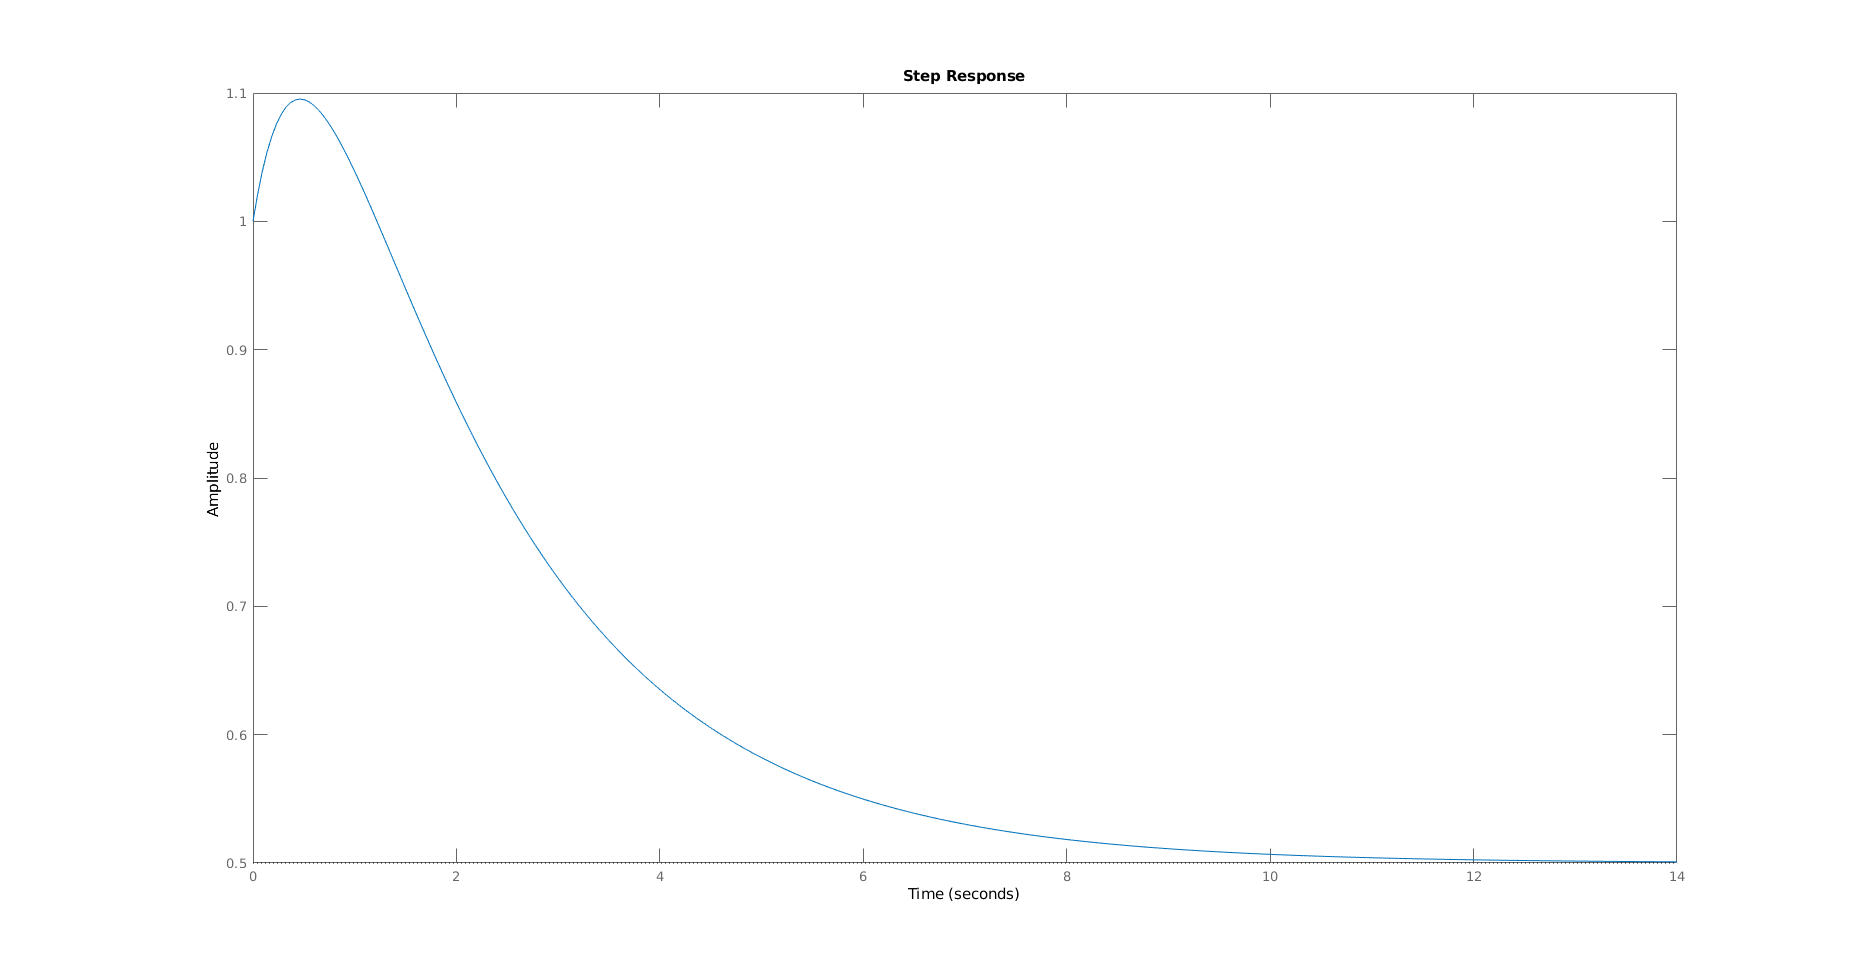
\includegraphics[width=\textwidth]{plot1.png}
	\captionsetup{labelformat=empty}
	\caption{Abb. 3-2.1: Sprungantwort für $R_1\neq R_2$}
\end{figure}
\subsection*{e)}
Beispielhaft wurden folgende Werte gewählt:
\begin{align*}
	R_1=2\Omega,\hspace{3pt}R_2=2\Omega,\hspace{3pt}C=0.5F,\hspace{3pt}L=2H
\end{align*}
Nullstellen:
\begin{align*}
	s_{n,1/2}=-1.0
\end{align*}
Pole:
\begin{align*}
	s_{p,1/2}=-1.0
\end{align*}
\begin{figure}[H]
	\centering
	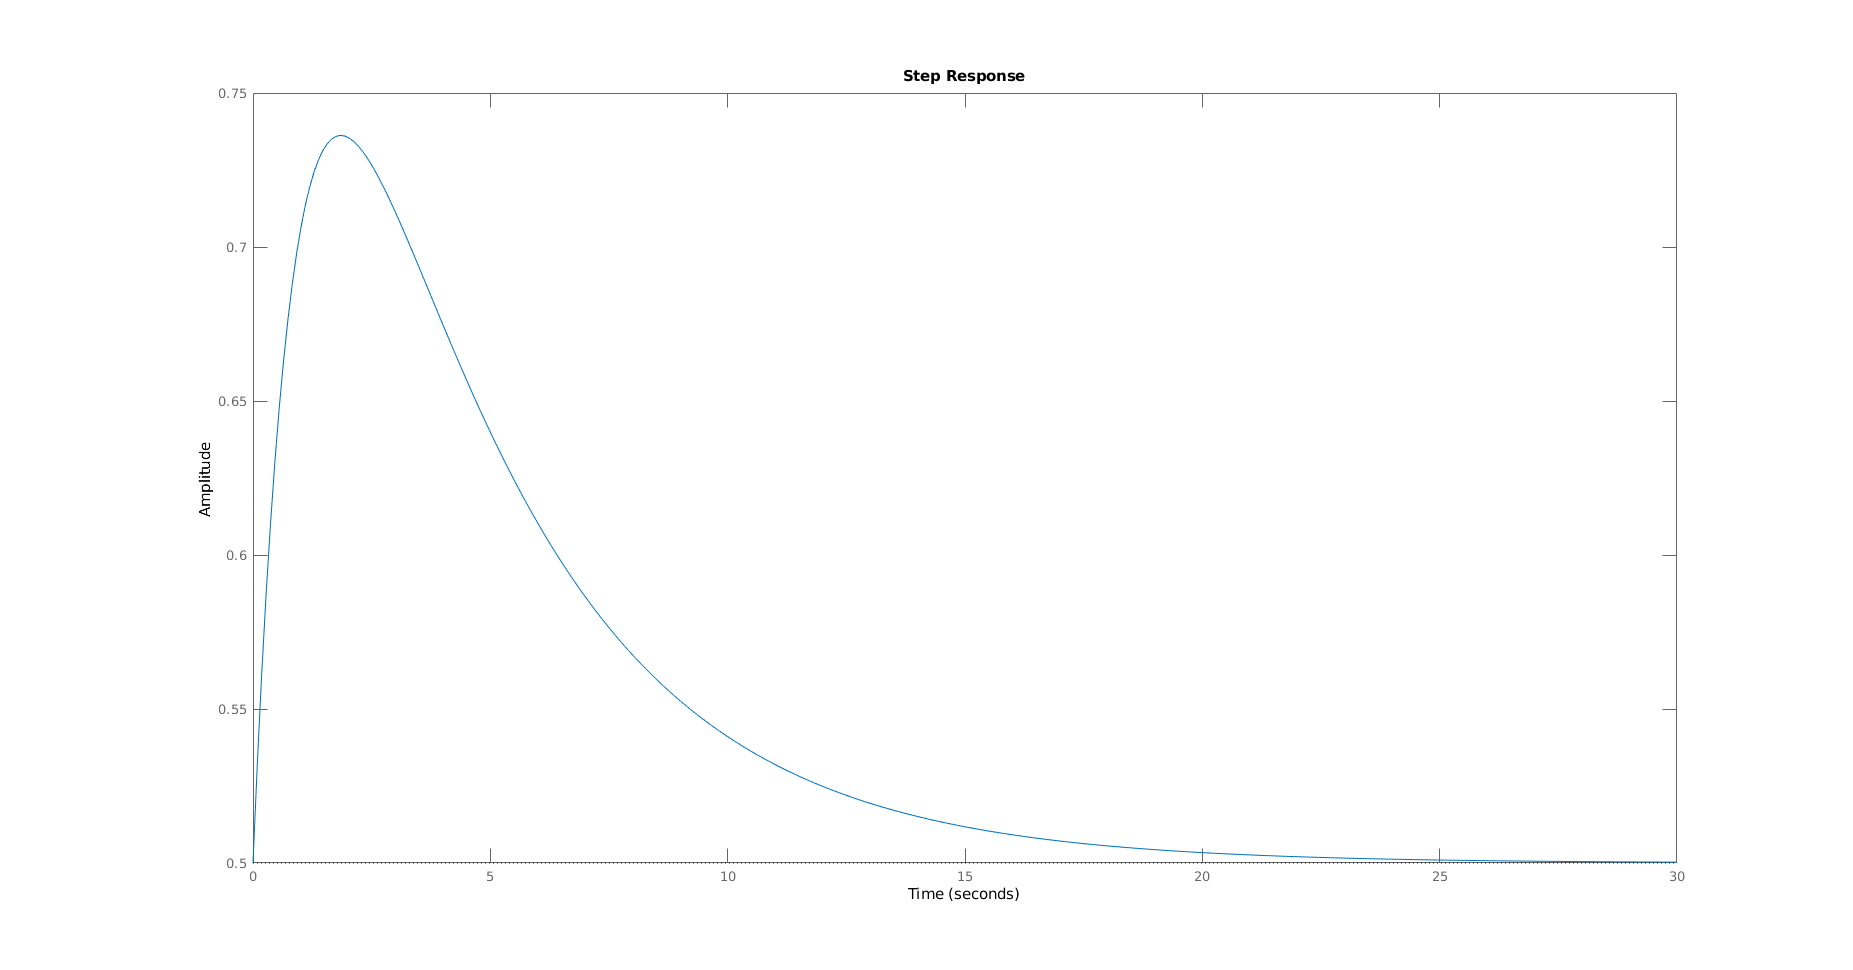
\includegraphics[width=\textwidth]{plot2.png}
	\captionsetup{labelformat=empty}
	\caption{Abb. 3-2.2: Sprungantwort für $R_1=R_2$}
\end{figure}
\end{document}
